\documentclass{article}

\usepackage{geometry}
\usepackage{amsmath}
\usepackage{graphicx, eso-pic}
\usepackage{listings}
\usepackage{hyperref}
\usepackage{multicol}
\usepackage{fancyhdr}
\pagestyle{fancy}
\fancyhf{}
\hypersetup{ colorlinks=true, linkcolor=black, filecolor=magenta, urlcolor=cyan}
\geometry{ a4paper, total={170mm,257mm}, top=10mm, right=20mm, bottom=20mm, left=20mm}
\setlength{\parindent}{0pt}
\setlength{\parskip}{0.3em}
\renewcommand{\headrulewidth}{0pt}

\rfoot{\thepage}
\fancyhf{} % sets both header and footer to nothing
\renewcommand{\headrulewidth}{0pt}
\lfoot{\textbf{Seleksi IEEEXtreme 17.0 ITB}}
\pagenumbering{gobble}

\fancyfoot[CE,CO]{\thepage}
\lstset{
    basicstyle=\ttfamily\small,
    columns=fixed,
    extendedchars=true,
    breaklines=true,
    tabsize=2,
    prebreak=\raisebox{0ex}[0ex][0ex]{\ensuremath{\hookleftarrow}},
    frame=none,
    showtabs=false,
    showspaces=false,
    showstringspaces=false,
    prebreak={},
    keywordstyle=\color[rgb]{0.627,0.126,0.941},
    commentstyle=\color[rgb]{0.133,0.545,0.133},
    stringstyle=\color[rgb]{01,0,0},
    captionpos=t,
    escapeinside={(\%}{\%)}
}

\begin{document}

\begin{center}

    
    \section*{Pixel Time} % ganti judul soal

    \begin{tabular}{ | c c | }
        \hline
        Batas Waktu  & 1s \\    % jangan lupa ganti time limit
        Batas Memori & 256MB \\  % jangan lupa ganti memory limit
        \hline
    \end{tabular}
\end{center}

\subsection*{Deskripsi}

Tendou Arisu adalah seorang siswi dari SMA Millenium yang tergabung dalam klub Game Development Department. Ia dan temannya Momoi sedang membuat sebuah game pixel baru yang bernama Tales Saga Chronicle 2. Pada pembuatan game tersebut Arisu ditugaskan untuk menjadi tester game yang telah dibuat. Pada game tersebut Arisu akan menjadi sebuah karakter yang terletak pada dunia paralel yang bernama dunia kartesius, dan karakter yang diperankan Arisu akan berada pada koordinat (0,0).\\

Pada game ini Momoi akan menempatkan N buah papan dengan sebuah papan direpresentasikan menggunakan $x_1, y_1, x_2, y_2$ yang mana ($x_1, y_1$) merupakan titik awal papan dan ($x_2, y_2$) merupakan titik akhir papan. Arisu akan diberikan sebuah senjata bernama \emph{Sword of Light: Supernova} yang merupakan senjata laser dengan daya tembak sangat besar sehingga akan menghancurkan dan menembus seluruh papan yang dilaluinya. Poin yang didapat Arisu dihitung berdasarkan banyaknya papan yang dihancurkan.\\

Ketika mencoba game tersebut Arisu penasaran berapa banyak poin yang bisa Ia dapatkan dalam sekali tembakan. Bantu Arisu menghitung berapa banyak poin yang bisa Ia dapatkan dalam sekali tembakan.\\

Notes: tidak ada garis papan yang akan memotong titik (0,0) jika garis tersebut dipanjangkan ataupun tidak

\subsection*{Format Masukan}

Input diawali dengan satu bilangan N ($1 \leq N \leq 10^5$) merepresentasikan jumlah papan yang ada.\\

Lalu untuk N baris berikutnya berisi $x_{i1}, y_{i1}, x_{i2}, y_{i2} (-10^6 \leq x_1, y_1, x_2, y_2 \leq 10^6)$ yang merepresentasikan papan ke-i.

\subsection*{Format Keluaran}

Berikan output berisi poin maksimal yang mungkin didapatkan Arisu dalam sekali tembakan.

\begin{multicols}{2}
\subsection*{Contoh Masukan}
\begin{lstlisting}
4
-2 9 6 5
0 5 10 3
2 -8 10 -4
-6 -6 0 -10
\end{lstlisting}
\columnbreak
\subsection*{Contoh Keluaran}
\begin{lstlisting}
2
\end{lstlisting}
\vfill
\null
\end{multicols}

\subsection*{Penjelasan}
Berikut ilustrasi dunia kartesius dimana karakter Arisu berada. Perhatikan garis yang ada pada gambar merupakan papan-papan yang disiapkan oleh Momoi.\\
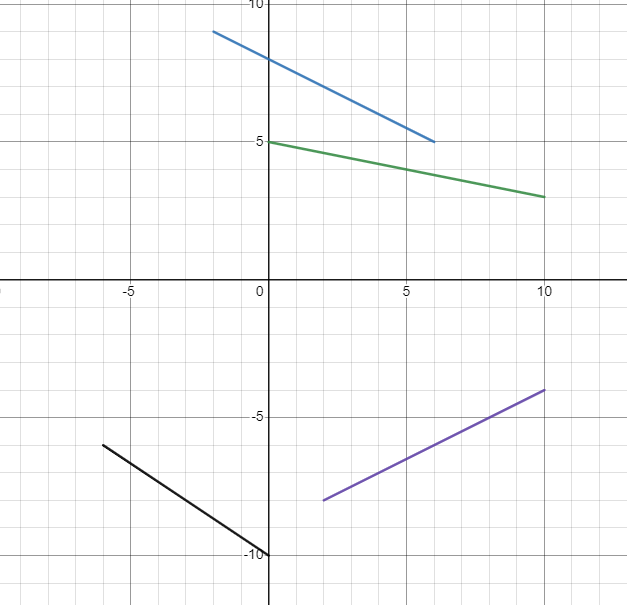
\includegraphics[scale=0.7]{desmos1}\\
Berikut adalah salah satu cara menembak yang menghasilkan poin terbanyak yaitu 2.\\
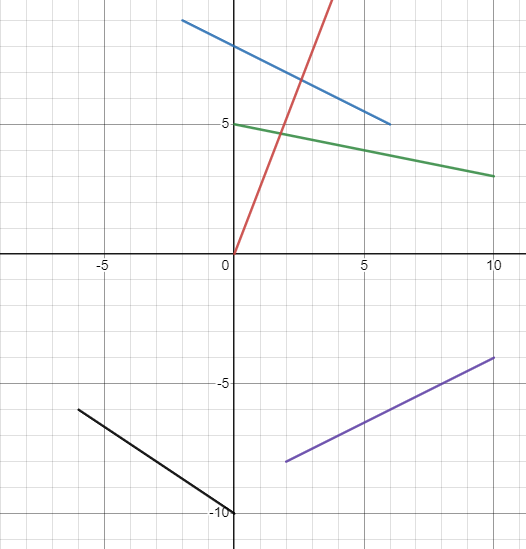
\includegraphics[scale=0.8]{desmos2}\\
Tembakan Arisu di ilustrasikan menggunakan garis berwarna merah.


\end{document}